\documentclass[a4paper,11pt]{article}
\usepackage{a4wide}
\usepackage{fullpage}
\usepackage[utf8x]{inputenc}
\usepackage[slovene]{babel}
\selectlanguage{slovene}
\usepackage[toc,page]{appendix}
\usepackage[pdftex]{graphicx}
\usepackage{setspace}
\usepackage{color}
\definecolor{light-gray}{gray}{0.95}
\usepackage{listings}
\usepackage{hyperref}
\usepackage{multirow}
\usepackage[table,xcdraw]{xcolor}
\renewcommand{\baselinestretch}{1.2}
\renewcommand{\appendixpagename}{Priloge}

\lstset{
language=Python,
basicstyle=\footnotesize,
basicstyle=\ttfamily\footnotesize\setstretch{1},
backgroundcolor=\color{light-gray},
}

\title{Seminar: Paralelizacija določanja vidnih odsekov črt}
\author{Primož Lavrič (63130133)}
\date{\today}

\begin{document}

\maketitle

\section{Uvod}

Cilj seminarja je bil zasnovati kar se da optimalni paralelni algoritem za reševanje problema vidnih črt na izbranih arhitekturah. Gre za geometrijski problem, pri katerem določamo vidni del vertikalnih črt iz opazovalčeve perspektive (v našem primeru se opazovalec lahko nahaja le v izhodišču koordinatnega sistema, zaradi poenostavitve problema). Za vse črte velja, da so neprekrivajoče in se nahajajo v prvem kvadrantu koordinatnega sistema, vsaka izmed črt ima eno končno točko na \textbf{x} osi koordinatnega sistema in je pravokotna na \textbf{x} os. Zaradi poenostavitve problema lahko vidni del posamezne črte izračunamo v odvisnosti od predhodnih s pomočjo kotne funkcije tangens. Velja $\tan \alpha =\frac{nasprotna\_kateta\ (Y)}{prilezna\_kateta\ (X)}$ torej za vsako črto, ki je vidna velja: $\frac{Y_{i-s}}{X_{i-s}} < \frac{Y_{i}}{X_{i}}$ za $1 <= s <= i$. Vidni odsek črte $i$ pa je definiran z $vis_{i} = Y_{i} - \frac{X_{i-1}}{Y_{i-1}} * X_{i}$

\begin{figure}[htbp]
\begin{center}
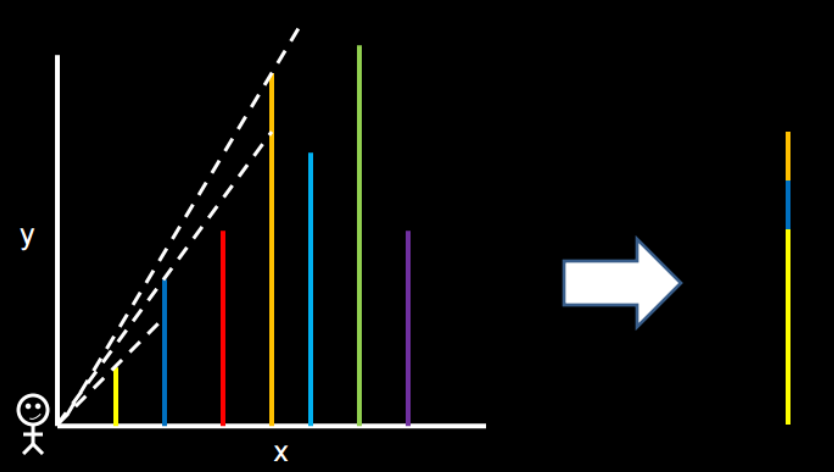
\includegraphics[scale=0.5]{slika-problema.png}
\caption{Shema problema.}
\label{slika1}
\end{center}
\end{figure}

\pagebreak
\section{Izbrane arhitekture in pristopi}

\subsection{Rešitev z uporabo PThread}
Sama implementacija s pomočjo PThread je nastala kot prototip GPU implementacije. Cilj implementacije je tem bolj optimizirati računanje maksimalnega elementa predpone (z njim določimo, če je zadnja črta, ki ustreza zadnjemu elementu predpone vidna oz. kakšen delež črte je viden). Pri snovanju učinkovitega algoritma za računanje predpon sem se zgledoval po Mark Harrisovem članku, ki opisuje učinkovito implementacijo "prefix sum" algoritma na arhitekturi Cuda\cite{bib:nvidiaPrefix}.

\noindent Glavna ideja te implementacije je zgraditi uravnoteženo binarno drevo čez vhodne podatke. Čez vpeto drevo nato izračunamo maksimalni element na poti do vsakega izmed vozlišč iz listov do korena in nazaj. Ta dva koraka imenujemo "up-sweep"\ref{slika2} in "down-sweep"\ref{slika3}. Ker je binarno drevo uravnoteženo, ima tako vpeto drevo $log(n)$ nivojev, na vsakem izmed nivojev pa $2^d$ vozlišč. Torej za izvršitev enega koraka ("up-sweep", "down-sweep") potrebujemo O(n-1) operacij (za vsako vozlišče enkrat izračunamo maksimalno vrendost). Za izračun maksimalnih predpon torej potrebujemo $2 * O(n-1)$ operacij. 

\noindent
Glede na zgornji opis je vredno omeniti, da se pri dani implementaciji ne uporablja dejansko binarno drevo, ampak to služi zgolj kot koncept, ki določa delo niti v posameznih korakih (izračuni na posameznem nivoju konceptualnega drevesa se lahko izvršijo paralelno).


\noindent
\textbf{Celotno implementacijo sestavljajo 4 koraki:}
\begin{enumerate}
\item Realociranje vektorja podanih višin na velikost $2^{ceil(log2(N))}$. Implementacija namreč zahteva, da je dvojiški logaritem velikosti podanega vektorja celo število. Čez vektor namreč želimo vpeti polno uravnoteženo dvojiško drevo.
\item Izračun razmerij višin črt in njihove oddaljenosti od opazovalca.
\item Nad izračunanim vektorjem razmerij $\vec{r}$ nato izvedemo zgoraj opisan algoritem ("prefix max scan"). Ta algoritem nam vrne vektor  $\vec{m}$ za katerega velja $\vec{m_i} = max(\vec{r_0}, \vec{r_1}, ..., \vec{r_{i-1}})$ za $i > 0$ in $\vec{m_0} = 0$.
\item V zadnjem koraku se izračunajo vidne višine s pomočjo vektorja $\vec{m}$, izračunanega v 3. koraku, vektorja višin $\vec{y}$ in vektorja oddaljenosti črt od opazovalca $\vec{x}$. Vektor vidnih višin je torej definiran kot $vis_{i} = \vec{y} - \vec{m} * \vec{x}$. Tu je vredno omeniti, da se ta korak izvede v zadnjem koraku down-sweepa (zaradi optimizacije dostopa do pomnilnika).
\end{enumerate} 

\begin{figure}[htbp]
\begin{center}
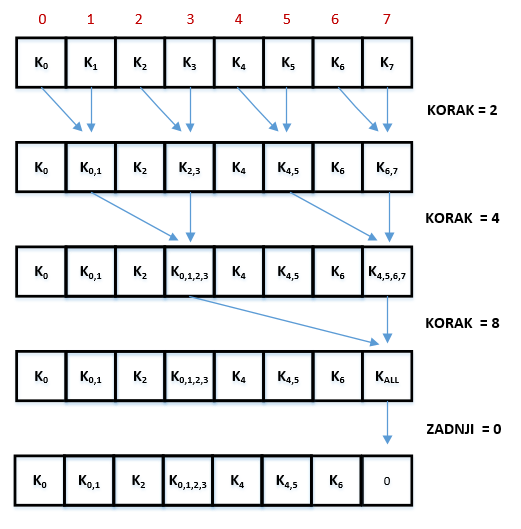
\includegraphics[scale=0.74]{up-sweep.png}
\caption{Primer "up-sweep" koraka.}
\label{slika2}
\end{center}
\end{figure}

\begin{figure}[htbp]
\begin{center}
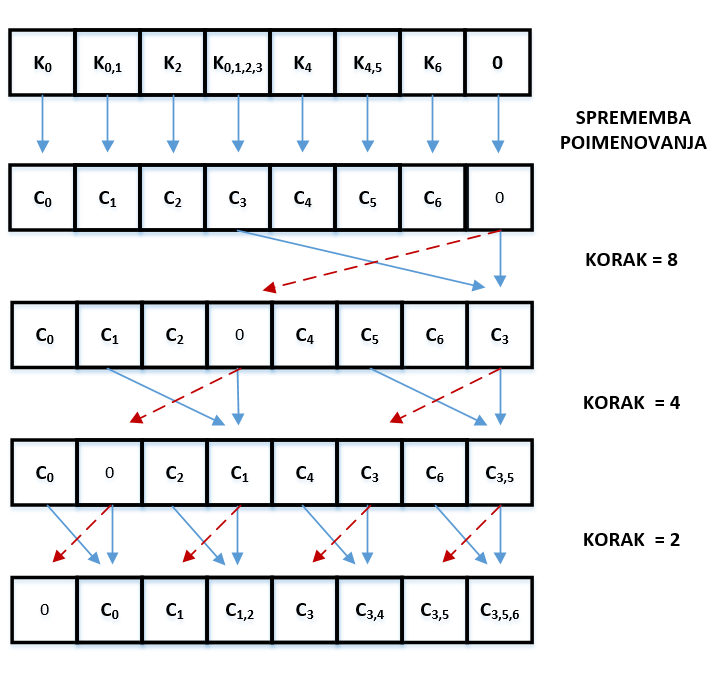
\includegraphics[scale=0.55]{down-sweep.png}
\caption{Primer "down-sweep" koraka.}
\label{slika3}
\end{center}
\end{figure}

\pagebreak
\subsection{Rešitev z uporabo OpenCL}
Implemetacija s pomočjo OpenCL se nekoliko razlikuje od implementacije s pomočjo pthread. Glavni razlog za razliko je sama arhitektura (ščepec se namreč izvaja na grafični procesni enoti GPE). Sam ščepec izvajajo delovne skupine, ki vsebujejo \textbf{N} niti. Tu se pojavi problem sinhronizacje, saj je na GPE mogoče sinhronizirati samo niti, ki se nahajajo znotraj ene delovne skupine, samih delovnih skupin pa ni mogoče sinhronizirati. Ker zgoraj opisana implementacija zahteva, da se nivoji vpetega drevesa poračunajo zaporedno, ni mogoče izračunati maksimalnih predpon vektorja večjega od maksimalne velikosti delovne skupine. Dani problem sem rešil tako, da probleme večje od velikosti delovne skupine razdelim na več podproblemov velikosti ene delovne skupine. Primer: za problem velikosti $4*W$, kjer je $W$ velikost delovne skupine, razdelim glavni problem na 4 podprobleme, ki jih rešujejo različne delovne skupine.

\noindent
Tu nastane naslednji problem, maksimalne predpone so namreč poračunane samo za posamezne podprobleme, zato je potrebno maksimalni element posameznega podproblema upoštevati v vseh naslednjih podproblemih, da bo globalni problem pravilno rešen. Tega sem se lotil tako, da shranim začasne maksimalne elemente posameznih podproblemov in nato v naslednjem ščepcu izračunam maksimalne predpone teh elementov. To rekurzivno ponavljam, dokler ni število maksimalnih elementov manjše od velikosti ene delovne skupine. Tedaj se rekurzivno vračam čez vse maksimalne elemente, pri katerih upoštevam maksimalne elemente njihovih predhodnih podproblemov (enostaven primer je prikazan na sliki \ref{slika4}). Po končanem propagiranju predhodnih podproblemov lahko sedaj poračunamo vidne višine posameznih črt.


\noindent
\textbf{Celotno implementacijo sestavlja 5 korakov (in 4 ščepci):}
\begin{enumerate}
\item Razčlenitev problema, računanje globine rekurzije in inicializacija potrebnih ščepcev.
\item Izvršitev prvega ščepca, ki izračuna razmerja, lokalno izvrši izračun maksimalnih predpon ter v vektor maksimalnih vrednosti podproblemov zapiše maksimalno vrednost poračunanega podproblema.
\item Izvršitev drugega ščepca (glede na velikost problema se lahko izvrši večkrat ali nikoli), vhod tega ščepca je vektor maksimalnih elementov predhodnega ščepca. Njegova naloga je, da nad tem vektorjem izvrši izračun maksimalnih predpon in v primeru, da je ščepec izvršilo več skupin, vsaka izmed skupin zapiše svojo maksimalno vrednost v naslednji vektor maksimalnih vrednosti podproblemov.
\item Izvršitev tretjega ščepca (glede na velikost problema se lahko izvrši večkrat ali nikoli), vhod tega ščepca je vektor maksimalnih predpon podproblemov. Naloga tega ščepca je, da pravilno propagira te predpone.
\item Izvršitev četrtega ščepca, naloga katerega je, da propagira zadnji vektor maksimalnih predpon podproblemov in nato izračuna dejanske vidne višine črt.

\end{enumerate}


\begin{figure}[htbp]
\begin{center}
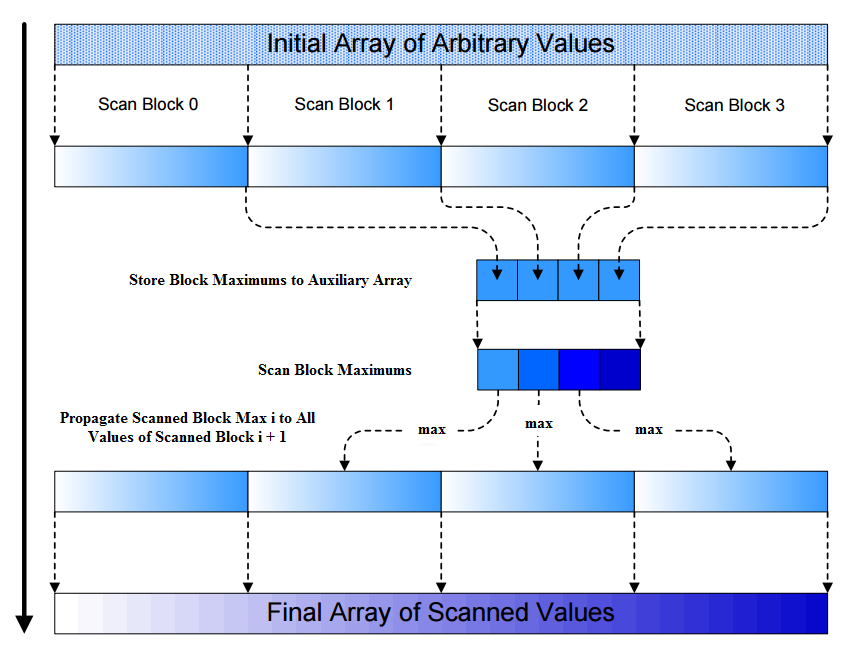
\includegraphics[scale=0.5]{max_scan_arbitary.png}
\caption{Primer maksimalnih predpon na problemu večjem od velikosti delovne skupine.}
\label{slika4}
\end{center}
\end{figure}

\pagebreak
\subsection{Rešitev z uporabo OpenMPI}
Implementacije algoritma s pomočjo OpenMPI sem se lotil nekoliko drugače. Zgoraj opisani pristop namreč zahteva veliko komunikacije, katero želimo pr uporabi OpenMPI minimizirati (zaradi veliko počasnejšega komunicranja med procesi čez omrežje). Glavna ideja implementacije je, da vsak izmed procesov dobi približno enak kos podatkov, katerega najprej sam sprocesira (izračuna kvociente in maksimalne predpone kvocientov). Ker je vsak kos podatkov odvisen od vseh predhodnih kosov, je potrebno upoštevati maksimalne kvociente vseh predhodnikov. Ta problem rešim tako, da vsak proces pošlje svoj maksimalni kvocient vsem naslednikom, ki nato poiščejo maksimalnega od vseh prejetih kvocientov. Ta kvocient nato propagirajo čez svoje kvociente (dokler ne naletijo na večji kvocient od prejetega). Vsak izmed procesov izračuna vidne višine, katere posreduje glavnemu procesu, ki jih združi v končno rešitev.

\noindent
\textbf{Celotno implementacijo sestavlja 7 korakov:}
\begin{enumerate}
\item Izračun razdelitve dela med procesi (izračun velikosti kosov, ki jih dobijo posamezni procesi).
\item Razpošiljanje kosov med vse delovne procese.
\item Izračun kvocientov in računanje maksimalnih predpon.
\item Posredovanje lokalnega maksimuma vsem naslednikom in sprejemanje lokalnih maksimumov vseh predhodnikov (izračun maksimalnega lokalnega maksimuma predhodnikov).
\item Propagiranje izračunanega maksimuma čez lokalne maksimalne predpone (dokler ne naleti do predpone večje od propagiranega maksimuma).
\item Vsak izmed procesov izračuna višine s pomočjo izračunanih maksimalnih predpon.
\item Združevanje rezultatov v glavnem procesu.
\end{enumerate}
\section{Rezultati}

\subsection{Sekvenčni algoritem}
Sekvenčno implementacijo sem stestiral z različnimi optimizacijami prevajalnika. Najbolj zanimva je O3 optimizacija, saj je sam faktor pohitritve 1.4, kar je primerljivo s paralelnimi implementacijami.

\begin{table}[h]
\centering
\begin{tabular}{|c|c|c|c|}
\hline
\rowcolor[HTML]{C0C0C0} 
\multicolumn{1}{|l|}{\cellcolor[HTML]{C0C0C0}\textbf{Velikost problema}} & \multicolumn{1}{l|}{\cellcolor[HTML]{C0C0C0}\textbf{Optimizacija}} & \multicolumn{1}{l|}{\cellcolor[HTML]{C0C0C0}\textbf{Čas izvajanja (s)}} & \multicolumn{1}{l|}{\cellcolor[HTML]{C0C0C0}\textbf{STD (s)}} \\ \hline
                                                                         & Od                                                                 & 0.3712                                                                  & 0.0036                                                                         \\ \cline{2-4} 
\multirow{-2}{*}{244 MB}                                                 & \cellcolor[HTML]{C0C0C0}{\color[HTML]{000000} O3}                  & \cellcolor[HTML]{C0C0C0}{\color[HTML]{000000} 0.2652}                   & \cellcolor[HTML]{C0C0C0}{\color[HTML]{000000} 0.0032}                          \\ \hline
                                                                         & Od                                                                 & 0.7391                                                                  & 0.0086                                                                         \\ \cline{2-4} 
\multirow{-2}{*}{488 MB}                                                 & \cellcolor[HTML]{C0C0C0}{\color[HTML]{000000} O3}                  & \cellcolor[HTML]{C0C0C0}{\color[HTML]{000000} 0.5282}                   & \cellcolor[HTML]{C0C0C0}{\color[HTML]{000000} 0.0041}                          \\ \hline
                                                                         & Od                                                                 & 1.4967                                                                  & 0.0248                                                                         \\ \cline{2-4} 
\multirow{-2}{*}{976 MB}                                                 & \cellcolor[HTML]{C0C0C0}{\color[HTML]{000000} O3}                  & \cellcolor[HTML]{C0C0C0}{\color[HTML]{000000} 1.0549}                   & \cellcolor[HTML]{C0C0C0}{\color[HTML]{000000} 0.0058}                          \\ \hline
                                                                         & Od                                                                 & 2.9973                                                                  & 0.0326                                                                         \\ \cline{2-4} 
\multirow{-2}{*}{1953 MB}                                                & \cellcolor[HTML]{C0C0C0}{\color[HTML]{000000} O3}                  & \cellcolor[HTML]{C0C0C0}{\color[HTML]{000000} 2.1071}                   & \cellcolor[HTML]{C0C0C0}{\color[HTML]{000000} 0.0122}                          \\ \hline
                                                                         & Od                                                                 & 6.1352                                                                  & 0.1273                                                                         \\ \cline{2-4} 
\multirow{-2}{*}{3906 MB}                                                & \cellcolor[HTML]{C0C0C0}{\color[HTML]{000000} O3}                  & \cellcolor[HTML]{C0C0C0}{\color[HTML]{000000} 4.3646}                   & \cellcolor[HTML]{C0C0C0}{\color[HTML]{000000} 0.1152}                          \\ \hline
\end{tabular}
\caption{Časi izvajanja sekvenčnega algoritma brez in z optimizacijo O3}
\label{my-label}
\end{table}

\begin{figure}[htbp]
\begin{center}
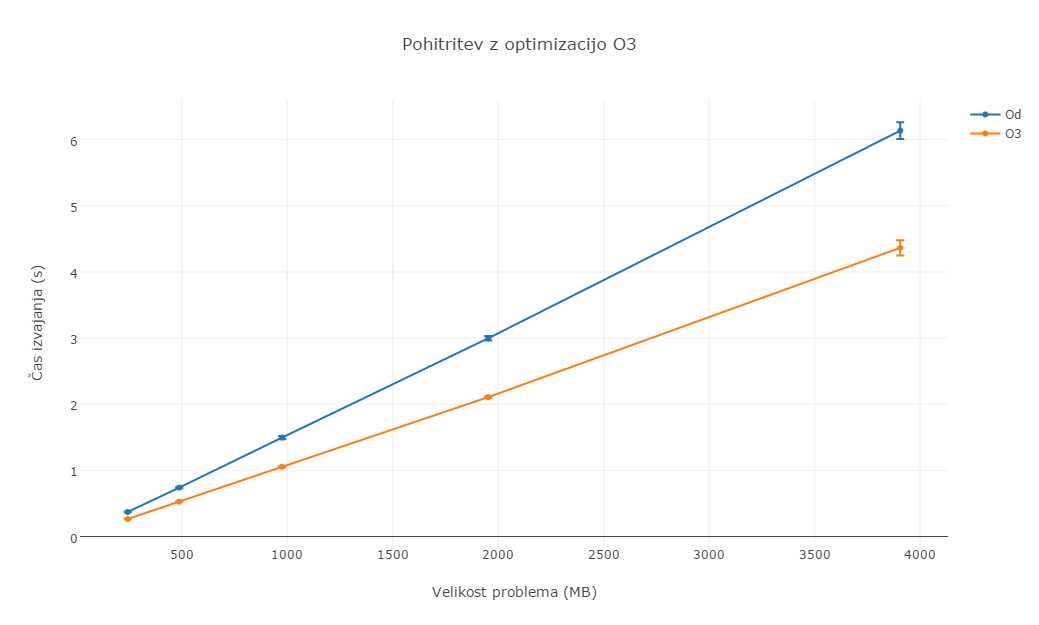
\includegraphics[scale=0.4]{o3-opt.png}
\caption{Pohitritev sekvenčnega algoritma z uporabo O3 optimizacije.}
\label{slika5}
\end{center}
\end{figure}

\pagebreak
\subsection{PThread}

Hitrost implementacije z uporabo PThread je na spodnji sliki\ref{slika6} primerjanja z ne optimirano implementacijo sekvečnega algoritma. Implementacija postane učinkovita šele pri uporabi 3 ali več niti in doseže faktor pohitritve okoli 2 na večjih problemih.

\begin{figure}[htbp]
\begin{center}
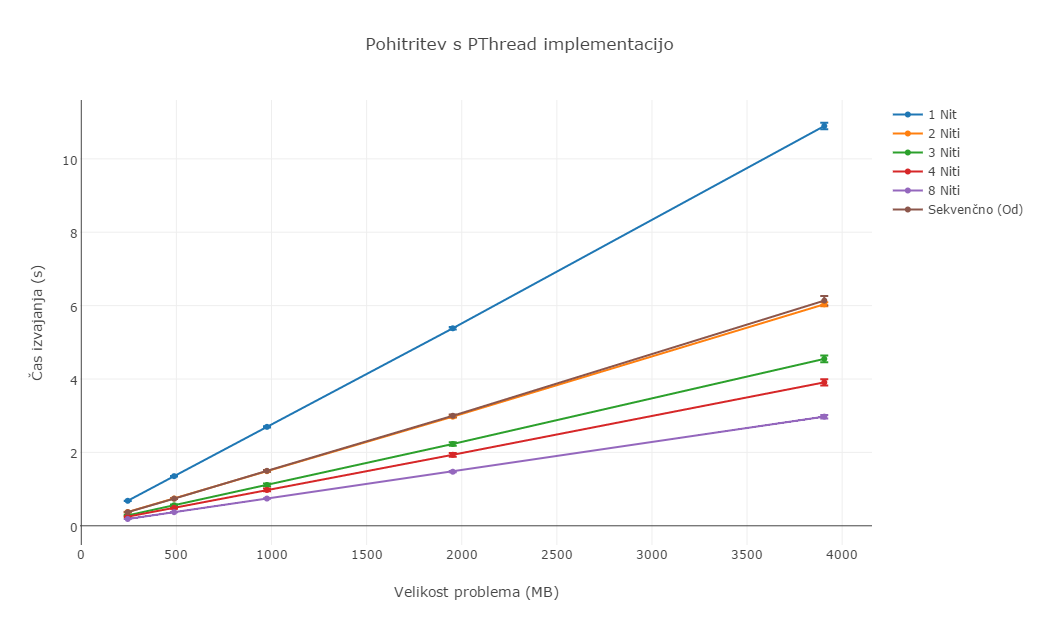
\includegraphics[scale=0.4]{pthread-opt.png}
\caption{Pohitritev sekvenčnega algoritma z uporabo PThread implementacije.}
\label{slika6}
\end{center}
\end{figure}

\begin{table}[h]
\centering
\begin{tabular}{|c|c|c|c|c|}
\hline
\rowcolor[HTML]{C0C0C0} 
\multicolumn{1}{|l|}{\cellcolor[HTML]{C0C0C0}\textbf{Velikost problema}} & \multicolumn{1}{l|}{\cellcolor[HTML]{C0C0C0}\textbf{Število niti}} & \multicolumn{1}{l|}{\cellcolor[HTML]{C0C0C0}\textbf{Čas izvajanja (s)}} & \multicolumn{1}{l|}{\cellcolor[HTML]{C0C0C0}\textbf{STD (s)}} & \multicolumn{1}{l|}{\cellcolor[HTML]{C0C0C0}\textbf{Faktor pohitritve}} \\ \hline
 & 1 & 0.6807 & 0.0021 & 0.55 \\ \cline{2-5} 
 & 2 & 0.3751 & 0.0062 & 0.99 \\ \cline{2-5} 
 & 3 & 0.2823 & 0.0181 & 1.31 \\ \cline{2-5} 
 & 4 & 0.2487 & 0.0150 & 1.49 \\ \cline{2-5} 
\multirow{-5}{*}{255 MB} & 8 & 0.1847 & 0.0027 & 2.01 \\ \hline
 
 & 1 & 1.3520 & 0.0075 & 0.55 \\ \cline{2-5} 
 & 2 & 0.7434 & 0.0087 & 0.99 \\ \cline{2-5} 
 & 3 & 0.5582 & 0.0237 & 1.32 \\ \cline{2-5} 
 & 4 & 0.4907 & 0.0238 & 1.51 \\ \cline{2-5} 
\multirow{-5}{*}{488 MB} & 8 & 0.3711 & 0.0044 & 1.99 \\ \hline
 
 & 1 & 2.6954 & 0.0170 & 0.56 \\ \cline{2-5} 
 & 2 & 1.4887 & 0.0180 & 1.01 \\ \cline{2-5} 
 & 3 & 1.1120 & 0.0378 & 1.35 \\ \cline{2-5} 
 & 4 & 0.9760 & 0.0366 & 1.53 \\ \cline{2-5} 
\multirow{-5}{*}{976 MB} & 8 & 0.7419 & 0.0083 & 2.02 \\ \hline
 
 & 1 & 5.3816 & 0.0347 & 0.56 \\ \cline{2-5} 
 & 2 & 2.9733 & 0.0298 & 1.01 \\ \cline{2-5} 
 & 3 & 2.2292 & 0.0458 & 1.34 \\ \cline{2-5} 
 & 4 & 1.9343 & 0.0523 & 1.55 \\ \cline{2-5} 
\multirow{-5}{*}{1953 MB} & 8 & 1.4729 & 0.0173 & 2.03 \\ \hline

 & 1 & 10.8940 & 0.0903 & 0.56 \\ \cline{2-5} 
 & 2 & 6.0351 & 0.0554 & 1.02 \\ \cline{2-5} 
 & 3 & 4.5477 & 0.0910 & 1.35 \\ \cline{2-5} 
 & 4 & 3.9081 & 0.0844 & 1.57 \\ \cline{2-5} 
\multirow{-5}{*}{3906 MB} & 8 & 2.9739 & 0.0481 & 2.06 \\ \hline
\end{tabular}
\caption{Časi izvajanja PThread implementacije in faktor pohitritve}
\label{pthread}
\end{table}

\pagebreak
\subsection{OpenCL (GPU)}

Hitrost implementacije z uporabp OpenCL (GPU) je na spodnji sliki\ref{slika7} primerjana z ne optimirano implementacijo sekvenčnega algoritma.
Sama implementacija dosega podobne pohitritve kot implementacija s pomočjo PThread z uporabo 8 niti. Implementacijo bi bilo mogoče še izbolšati z optimiranjem ščepca za računanje maksimalnih predpon (preprečevanje pomnilniških kolizij).

\begin{table}[h]
\centering
\begin{tabular}{|c|c|c|c|}
\hline
\rowcolor[HTML]{C0C0C0} 
\multicolumn{1}{|l|}{\cellcolor[HTML]{C0C0C0}\textbf{Velikost problema}} & \multicolumn{1}{l|}{\cellcolor[HTML]{C0C0C0}\textbf{Čas izvajanja (s)}} & \multicolumn{1}{l|}{\cellcolor[HTML]{C0C0C0}\textbf{STD (s)}} & \multicolumn{1}{l|}{\cellcolor[HTML]{C0C0C0}\textbf{Faktor pohitritve)}} \\ \hline
244 MB & 0.2033 & 0.0097 & 1.83 \\ \hline
488 MB & 0.3929 & 0.0122 & 1.88 \\ \hline
976 MB & 0.7423 & 0.1323 & 2.02 \\ \hline
1953 MB & 1.4794 & 0.0251 & 2.03 \\ \hline
3906 MB & 2.8249 & 0.1055 & 2.17 \\ \hline
\end{tabular}
\caption{Časi izvajanja OpenCL (GPU) implementacije ter faktor pohitritve}
\label{my-label}
\end{table}

\begin{figure}[htbp]
\begin{center}
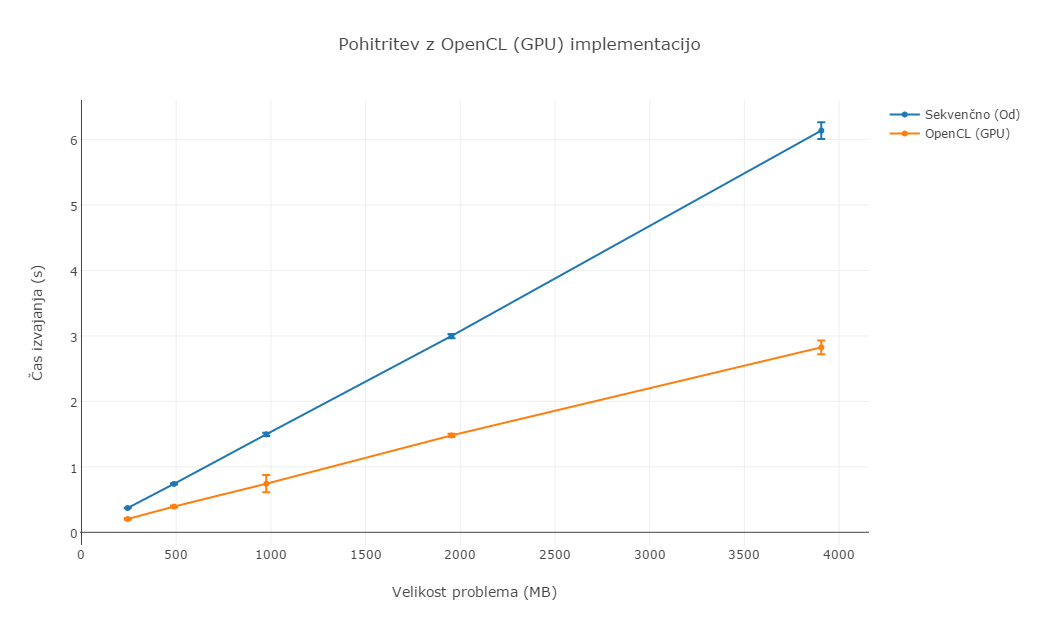
\includegraphics[scale=0.4]{gpu-opt.png}
\caption{Pohitritev sekvenčnega algoritma z uporabo OpenCL GPU implementacije.}
\label{slika7}
\end{center}
\end{figure}

\subsection{OpenMPI (Gruča)}
Implementacija s pomočjo OpenMPI se ni izkazala za najboljšo. Sama hitrost izračuna se je namreč zmanjšala v primerjavi z sekvenčnim algoritmom (pri tem velja omenita, da imata testna sistema različne performanse). Časi izvajanja so prikazani v spodnji tabeli \ref{openMPI}

% Please add the following required packages to your document preamble:
% \usepackage{multirow}
% \usepackage[table,xcdraw]{xcolor}
% If you use beamer only pass "xcolor=table" option, i.e. \documentclass[xcolor=table]{beamer}
\begin{table}[]
\centering
\begin{tabular}{|c|c|c|c|c|}
\hline
\rowcolor[HTML]{C0C0C0} 
\multicolumn{1}{|l|}{\cellcolor[HTML]{C0C0C0}\textbf{Velikost problema}} & \multicolumn{1}{l|}{\cellcolor[HTML]{C0C0C0}{\color[HTML]{343434} \textbf{Št. procesov}}} & \multicolumn{1}{l|}{\cellcolor[HTML]{C0C0C0}\textbf{Čas izvajanja (s)}} & \multicolumn{1}{l|}{\cellcolor[HTML]{C0C0C0}\textbf{STD (s)}} & \multicolumn{1}{l|}{\cellcolor[HTML]{C0C0C0}{\color[HTML]{343434} \textbf{Faktor pohitritve}}} \\ \hline
 & 4 & 2.6416 & 0.0043 & / \\ \cline{2-5} 
 & 8 & 2.5953 & 0.0819 & / \\ \cline{2-5} 
 & 16 & 2.8431 & 0.1636 & / \\ \cline{2-5} 
\multirow{-4}{*}{244 MB} & 32 & 3.2984 & 0.1675 & / \\ \hline
 & 4 & 5.2897 & 0.0109 & / \\ \cline{2-5} 
 & 8 & 5.1806 & 0.0750 & / \\ \cline{2-5} 
 & 16 & 5.1641 & 0.7982 & / \\ \cline{2-5} 
\multirow{-4}{*}{488 MB} & 32 & 5.7784 & 0.2177 & / \\ \hline
 & 4 & 10.5799 & 0.0155 & / \\ \cline{2-5} 
 & 8 & 10.3392 & 0.0882 & / \\ \cline{2-5} 
 & 16 & 10.3010 & 0.1194 & / \\ \cline{2-5} 
\multirow{-4}{*}{976 MB} & 32 & 10.5566 & 0.2565 & / \\ \hline
 & 4 & 21.1703 & 0.0325 & / \\ \cline{2-5} 
 & 8 & 20.6369 & 0.1676 & / \\ \cline{2-5} 
 & 16 & 20.3945 & 0.1292 & / \\ \cline{2-5} 
\multirow{-4}{*}{1953 MB} & 32 & 20.5796 & 0.2002 & / \\ \hline
\end{tabular}
\caption{časi izvajanja implementacije z uporabo OpenMPI na IJS gruči}
\label{openMPI}
\end{table}

\section{Testni sistem}
Sekvenčna, PThread in OpenCL implementacije so bile testirane na sistemu:
\begin{itemize}
\item Procesor: Intel i7 6700K 4.2 GHz
\item Ram: 16GB
\item GPU: Nvidia gtx 980ti
\end{itemize}
OpenMPI implementacija pa je bila testirana na IJS-jevi gruči (podana je specifikacija računalnikov):
\begin{itemize}
\item Procesor: Intel Xeon E5520 2.27 GHz
\item Ram: 8GB
\end{itemize}
\pagebreak

\begin{thebibliography}{99}
\bibitem{bib:nvidiaPrefix} Harris, Mark, Shubhabrata Sengupta, and John D. Owens. "Parallel prefix sum (scan) with CUDA." GPU gems 3.39 (2007): 851-876.
\end{thebibliography}


\end{document}
